\documentclass{article}

\usepackage[paperwidth=6.5in,paperheight=4.6in,margin=0in]{geometry}
\usepackage{tikz}
\usepackage[T1]{fontenc}
\usepackage{helvet}
\renewcommand{\familydefault}{\sfdefault}
\pagestyle{empty}

\definecolor{ink}{HTML}{0F172A}
\definecolor{muted}{HTML}{475569}
\definecolor{grid}{HTML}{E2E8F0}
\definecolor{panelbg}{HTML}{F8FAFC}
\definecolor{grpo}{HTML}{F59E0B}
\definecolor{topomcpo}{HTML}{2563EB}

\newcommand{\titlefont}{\fontsize{10}{11}\selectfont}
\newcommand{\tickfont}{\fontsize{7}{7.5}\selectfont}
\newcommand{\labelfont}{\fontsize{7.4}{8.0}\selectfont}
\newcommand{\legendfont}{\fontsize{8}{8.5}\selectfont}

\newcommand{\metricpanel}[6]{%
  \draw[fill=panelbg, draw=none] (#1,#2) rectangle ++(2.95,1.78);
  \node[anchor=west, text=ink, font=\bfseries\titlefont] at (#1+0.10,#2+1.55) {#3};
  \foreach \tick/\label in {#6} {%
    \pgfmathsetmacro{\yy}{#2+0.38+(\tick-#4)/(#5-#4)*1.00}
    \draw[grid, line width=0.9pt] (#1+0.48,\yy) -- (#1+2.72,\yy);
    \node[anchor=east, text=muted, font=\tickfont] at (#1+0.40,\yy) {\label};
  }
  \draw[grid, line width=0.9pt] (#1+0.48,#2+0.38) -- (#1+0.48,#2+1.38);
  \draw[grid, line width=0.9pt] (#1+0.48,#2+0.38) -- (#1+2.72,#2+0.38);
  \node[anchor=north, text=ink, font=\tickfont] at (#1+1.10,#2+0.27) {GRPO};
  \node[anchor=north, text=ink, font=\tickfont] at (#1+2.02,#2+0.27) {Topo-MCPO};
}

\newcommand{\barpair}[8]{%
  \pgfmathsetmacro{\base}{#2+0.38}
  \pgfmathsetmacro{\gheight}{(#5-#3)/(#4-#3)*1.00}
  \pgfmathsetmacro{\theight}{(#6-#3)/(#4-#3)*1.00}
  \pgfmathsetmacro{\gtop}{\base+\gheight}
  \pgfmathsetmacro{\ttop}{\base+\theight}
  \draw[fill=grpo, draw=white, line width=1.2pt] (#1+0.86,\base) rectangle (#1+1.34,\gtop);
  \draw[fill=topomcpo, draw=white, line width=1.2pt] (#1+1.78,\base) rectangle (#1+2.26,\ttop);
  \node[anchor=south, text=ink, font=\bfseries\labelfont] at (#1+1.10,\gtop+0.03) {#7};
  \node[anchor=south, text=ink, font=\bfseries\labelfont] at (#1+2.02,\ttop+0.03) {#8};
}

\begin{document}
\noindent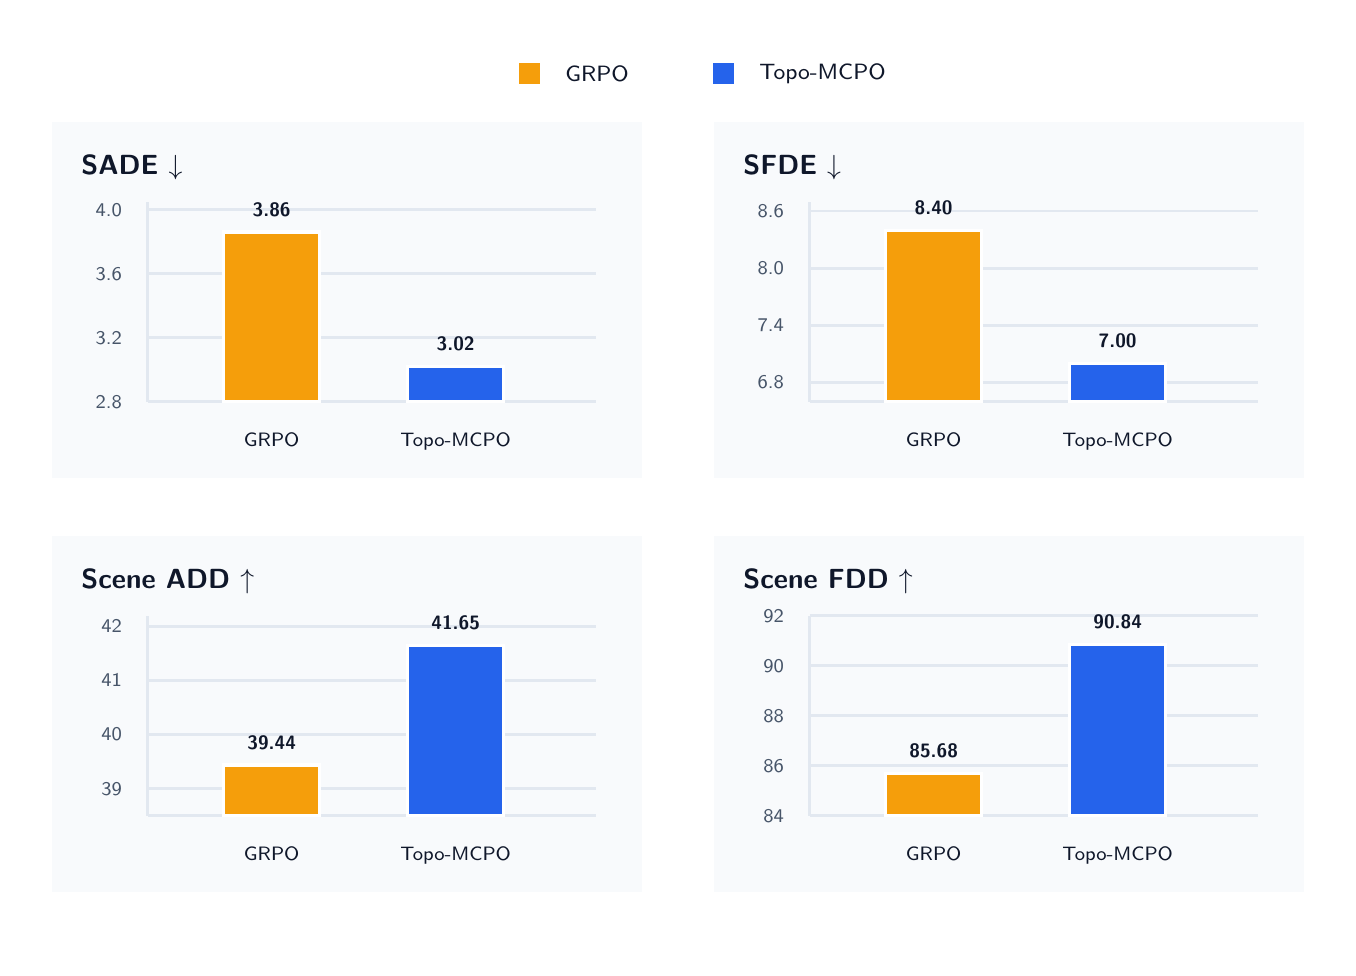
\begin{tikzpicture}[x=1in,y=1in]
  \fill[white] (0,0) rectangle (6.5,4.6);

  % Legend, matched to Figure 4's compact top-centered style.
  \draw[fill=grpo, draw=white, line width=1.0pt] (2.45,4.31) rectangle ++(0.12,0.12);
  \node[anchor=west, text=ink, font=\legendfont] at (2.64,4.37) {GRPO};
  \draw[fill=topomcpo, draw=white, line width=1.0pt] (3.42,4.31) rectangle ++(0.12,0.12);
  \node[anchor=west, text=ink, font=\legendfont] at (3.61,4.37) {Topo-MCPO};

  % Top row: all-agent displacement under all-label interventions.
  \metricpanel{0.12}{2.35}{SADE $\downarrow$}{2.8}{4.05}{2.8/2.8,3.2/3.2,3.6/3.6,4.0/4.0}
  \barpair{0.12}{2.35}{2.8}{4.05}{3.86}{3.02}{3.86}{3.02}

  \metricpanel{3.43}{2.35}{SFDE $\downarrow$}{6.6}{8.7}{6.8/6.8,7.4/7.4,8.0/8.0,8.6/8.6}
  \barpair{3.43}{2.35}{6.6}{8.7}{8.40}{7.00}{8.40}{7.00}

  % Bottom row: semantic coverage/diversity under the same all-label evaluation.
  \metricpanel{0.12}{0.28}{Scene ADD $\uparrow$}{38.5}{42.2}{39/39,40/40,41/41,42/42}
  \barpair{0.12}{0.28}{38.5}{42.2}{39.44}{41.65}{39.44}{41.65}

  \metricpanel{3.43}{0.28}{Scene FDD $\uparrow$}{84.0}{92.0}{84/84,86/86,88/88,90/90,92/92}
  \barpair{3.43}{0.28}{84.0}{92.0}{85.68}{90.84}{85.68}{90.84}
\end{tikzpicture}
\end{document}
